\documentclass[ENG]{TFUOC}%IB: CASTELLÀ, CAT: CATALÀ, ENG: ENGLISH

% Robust line breaks for long URLs/DOIs in references and text
\PassOptionsToPackage{hyphens}{url}
\usepackage{xurl}
\usepackage{microtype}

% Prevent right-margin overflow (overfull hboxes) in difficult lines
\emergencystretch=3em

% Espacio vertical entre párrafos
\setlength{\parskip}{0.6em}   % prueba 0.4em–1em
\setlength{\parindent}{0pt}   % opcional: sin sangría de primera línea

%Introduce Work Data
\title{Módulo 1 - Definición y planificación del trabajo final}
\titcrt{M1 - Definición y planificación del TFM} %Short title to appear in header
\author{Albert Gallego Jiménez}
\date{\today}

\nomPDC{Carlos Cabezas Rabadán and Joaquín Torres Sospedra}
\nomPRA{David Masip Rodó}
\titulac{MSc in Data Science}
\area{Area 4: Pattern Recognition and Computer Vision in Applied Sciences - Geographic Information Systems, satellite images and geopositioning}
\idioma{English}
\credits{15}
\parcla{Earth Observation, Satellite imagery, Coastal Remote Sensing, Semantic Segmentation, Spectral Indices, Water Segmentation}

\licenc{ccBy}
%Possible licenses
%ccByNcNd
%ccByNcSa
%ccByNc
%ccByNd
%ccBySa
%ccBy
%GNU
%copyright

\begin{document}

% This command generates the title page, license, work card and abstract pages
\estructura

\tableofcontents

\chapter{Proposed title}
Comparative Evaluation of Satellite Image Segmentation Methods for Coastline Extraction: Spectral Indices vs. Deep Learning.

\chapter{Keywords}
Earth Observation, Satellite imagery, Coastal Remote Sensing, Semantic Segmentation, Spectral Indices, Water Segmentation.

\chapter{Abstract}
Accurate coastline extraction using high-frequency satellite data like Sentinel-2 is a cornerstone of modern coastal engineering, but current automated methods face severe limitations. Environments characterized by large intertidal zones and complex hydrodynamics induce spectral confusion among water, wave foam, and wet sand. This project aims to assess if state-of-the-art Deep Learning models can overcome the shortcomings of classical pixel-based remote sensing techniques.

The methodology revolves around creating a high-quality, AI-annotated Ground Truth dataset covering two morphodynamically distinct locations (Cantabrian and Mediterranean coasts) to train and test advanced semantic segmentation models. These models will be strictly benchmarked against established baselines, which rely on the automatic Otsu thresholding of spectral indices such as the Normalized Difference Water Index (NDWI) and Modified NDWI (MNDWI). To capture both the correct classification of pixels and the physical accuracy of the shoreline, the evaluation will be twofold: utilizing standard computer vision metrics, like Intersection over Union (IoU) and Dice Coefficient, alongside sub-pixel geometric validation (mean Euclidean distance). Ultimately, this research will quantify the performance degradation of each method under adverse conditions and their cross-site transferability, defining the most robust approach for future coastal monitoring frameworks.

\chapter{Description of the proposal and justification of its interest and relevance}
Coastal regions are among the most dynamic and socioeconomically vital areas on Earth. Accurate shoreline detection is essential for monitoring erosion and planning coastal defense strategies. This task is increasingly being addressed through satellite remote sensing, where missions such as Sentinel-2 offer high-frequency and multi-decadal data for coastal morphological characterization \cite{vitousek_future_2023}. Currently, established frameworks like CoastSat \cite{vos_coastsat_2019}, SHOREX \cite{sanchez-garcia_efficient_2020}, and CASSIE \cite{almeida_coastal_2021} have successfully implemented workflows to define satellite-derived waterlines, providing low-cost information to track shoreline evolution across various scales.

However, these traditional methods based on spectral index thresholds often struggle with "noise," such as wave foam in swash zones and mixed pixels at the water-land interface. This is particularly evident on the Cantabrian coast, where high tides create a large intertidal area in which differences in water saturation in the sand can hinder waterline detection (see Figure~\ref{fig:misidentification_example}). Consequently, there is a clear need to explore more robust, context-aware approaches like Deep Learning to overcome the spectral confusion inherent in these highly dynamic environments.

\begin{figure}[!htbp]
    \centering
    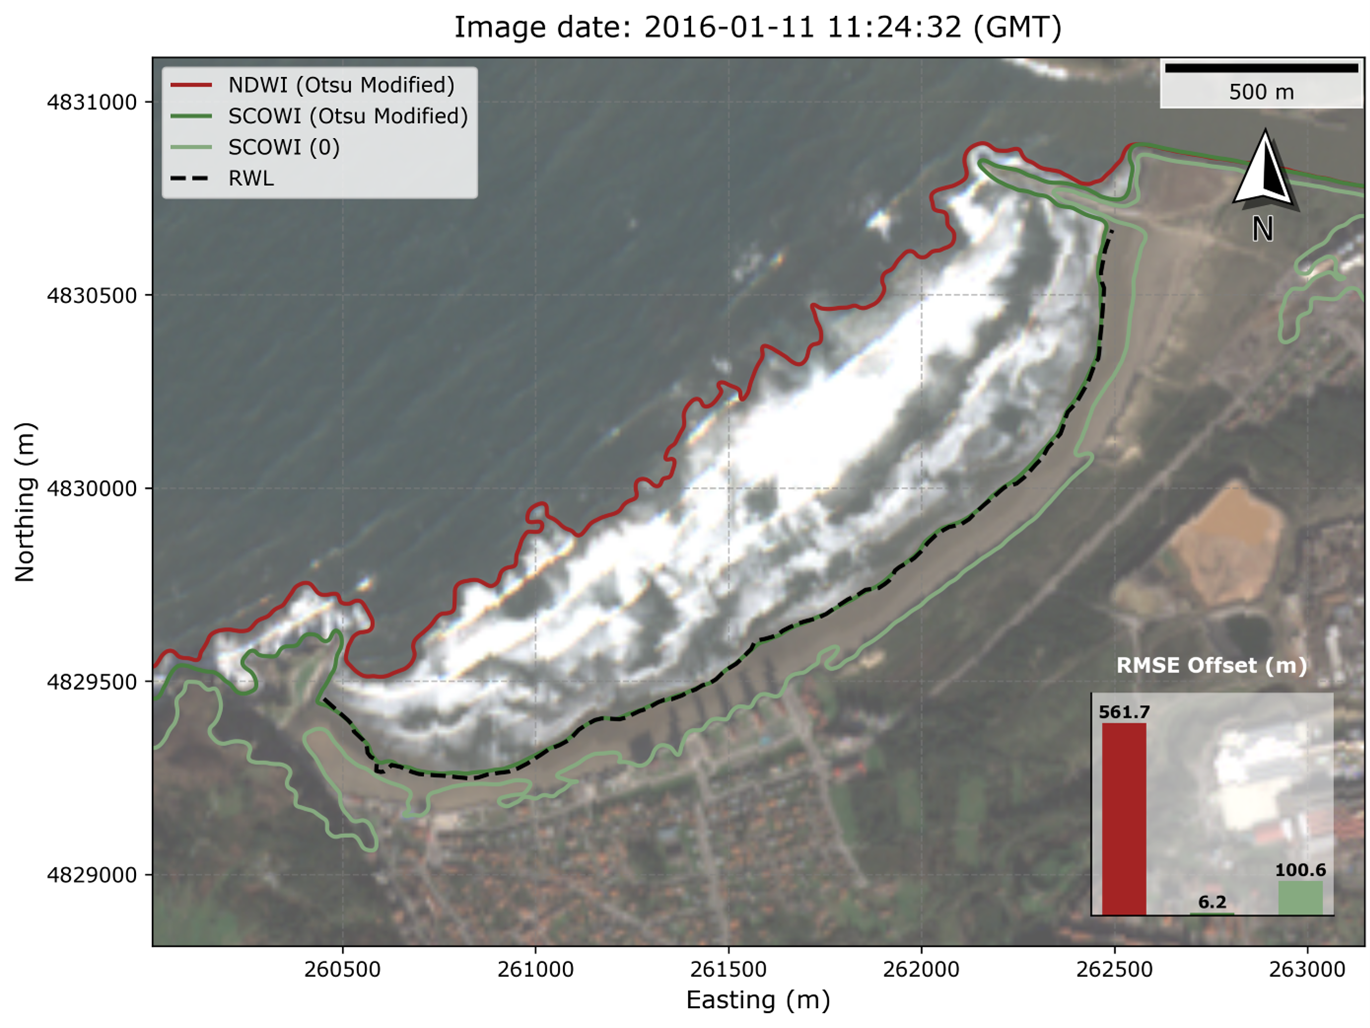
\includegraphics[width=15truecm]{shoreline_misidentification_example.png}
    \caption{Examples of shoreline misidentification in a macrotidal beach (adapted from \cite{cabezas_site-specific_2026})}
    \label{fig:misidentification_example}
\end{figure}

This proposal is relevant because it seeks to bridge the gap between classical remote sensing and modern computer vision by providing a quantified comparison of the accuracy gained by using deep learning models versus traditional spectral methods.

\chapter{Explanation of personal motivation}
Beyond my academic path in this master’s program, I currently work as a Coastal Engineer, specifically focusing on coastal monitoring through remote sensing and satellite imagery. My professional experience has provided me with a deep understanding of coastal dynamics; however, it has also exposed the technical limitations of traditional engineering tools when dealing with highly dynamic environments.

To address this, I aim to implement Deep Learning as it represents a significant scientific advancement over current pixel-based methods. Unlike traditional indices that rely on rigid thresholds, these models learn spatial context and complex textures, allowing them to resolve the spectral confusion between water, foam, and wet sand.

\chapter{Definition of objectives (primary and secondary)}
\noindent\textbf{Primary Objective:}
\begin{itemize}
    \item To perform a comprehensive benchmarking analysis between traditional spectral-based thresholding and Deep Learning-based semantic segmentation for coastline extraction.
\end{itemize}

\noindent\textbf{Secondary Objectives:}
\begin{itemize}
    \item To generate a high-quality "Ground Truth" dataset of coastal masks using AI-assisted annotation (SAM) \cite{kirillov_segment_2023}.
    \item To evaluate the performance degradation of each method under adverse conditions (foam, differences in sand moisture content, and clouds).
    \item To assess the transferability of trained models between different coastal typologies (Cantabrian vs. Mediterranean).
\end{itemize}

\chapter{Description of the methodology used in the development of the project}
The methodology is structured into four main phases as illustrated in the workflow diagram (Figure~\ref{fig:workflow}):
\begin{enumerate}
    \item \textbf{Data Acquisition:} Downloading Sentinel-2 Level-2A (atmospherically corrected) products from Google Earth Engine, covering the period 2015–2025. A built-in cloud detection algorithm will be applied as an initial filter to discard obstructed scenes, utilizing the remaining available cloud-free images.
    \item \textbf{Preprocessing \& Labelling:} Calculation of spectral indices (NDWI, MNDWI). Generation of Ground Truth masks using the Segment Anything Model (SAM) through an interactive annotation tool \cite{bhattiprolu_digitalsreeni_2026}.
    \item \textbf{Model Implementation:}
    \begin{itemize}
        \item \textit{Baseline:} Automatic Otsu thresholding applied to spectral indices.
        \item \textit{Deep Learning:} {\sloppy Training semantic segmentation models like U-Net \cite{navab_u-net_2015} or SegFormer \cite{xie_segformer_2021}. Model training will be run locally on an NVIDIA RTX 3060 GPU, with an institutional computing cluster (2 nodes, 2x NVIDIA A30 each) available for scaling if required.}
    \end{itemize}
    \item \textbf{Evaluation:} Comparison using pixel-based metrics (IoU, Dice) and geometric validation (calculating the mean Euclidean distance between the predicted and real coastline).
\end{enumerate}

\begin{figure}[!htbp]
    \centering
    \includegraphics[width=\linewidth]{Methodological_Workflow.png}
    \caption{Schematic representation of the methodological workflow.}
    \label{fig:workflow}
\end{figure}

\chapter{Research plan}
The project is planned to be developed over a 5-month period (including the thesis defence), structured into the following tasks as shown in the Gantt chart (Figure~\ref{fig:gantt}). Additionally, project management software such as Trello or MS Planner will be used to track and control the tasks at a more specific level:
\begin{itemize}
    \item \textbf{Task 1:} Literature review, selection of study sites (beaches), and satellite images download.
    \begin{itemize}
        \item Literature review on traditional methods for satellite-derived coastline extraction.
        \item Literature review on Deep Learning models applied to coastal monitoring.
        \item Satellite images download for Beach 1 (Cantabrian environment).
        \item Satellite images download for Beach 2 (Mediterranean environment).
    \end{itemize}
    \item \textbf{Task 2:} Calculation of spectral indices and generation of Ground Truth masks.
    \begin{itemize}
        \item Preparation of the GitHub repository structure for the project's codebase.
        \item Calculation of spectral indices (e.g., NDWI, MNDWI).
        \item Create false-color composites to assist in the annotation process.
        \item Ground Truth generation through AI-assisted annotation of the dataset.
    \end{itemize}
    \item \textbf{Task 3:} Model implementation: Development of baseline and Deep Learning architectures.
    \begin{itemize}
        \item Application of automatic thresholding to spectral indices to set baseline models.
        \item Selection, development, and training of Deep Learning architectures.
        \item Application of contouring algorithms to extract shorelines at sub-pixel precision.
    \end{itemize}
    \item \textbf{Task 4:} Statistical analysis of results, benchmarking across different algorithms, and final evaluation.
    \begin{itemize}
        \item Pixel-based metrics evaluation (e.g., IoU, Dice Coefficient).
        \item Geometric validation by calculating the mean Euclidean distance between predicted and real shorelines.
        \item Comparison of performance under adverse conditions (foam, wet sand) and transferability assessment.
    \end{itemize}
    \item \textbf{Task 5:} Drafting report and interim deliveries.
    \item \textbf{Task 6:} Progress meetings with directors.
\end{itemize}

\begin{figure}[!htbp]
    \centering
    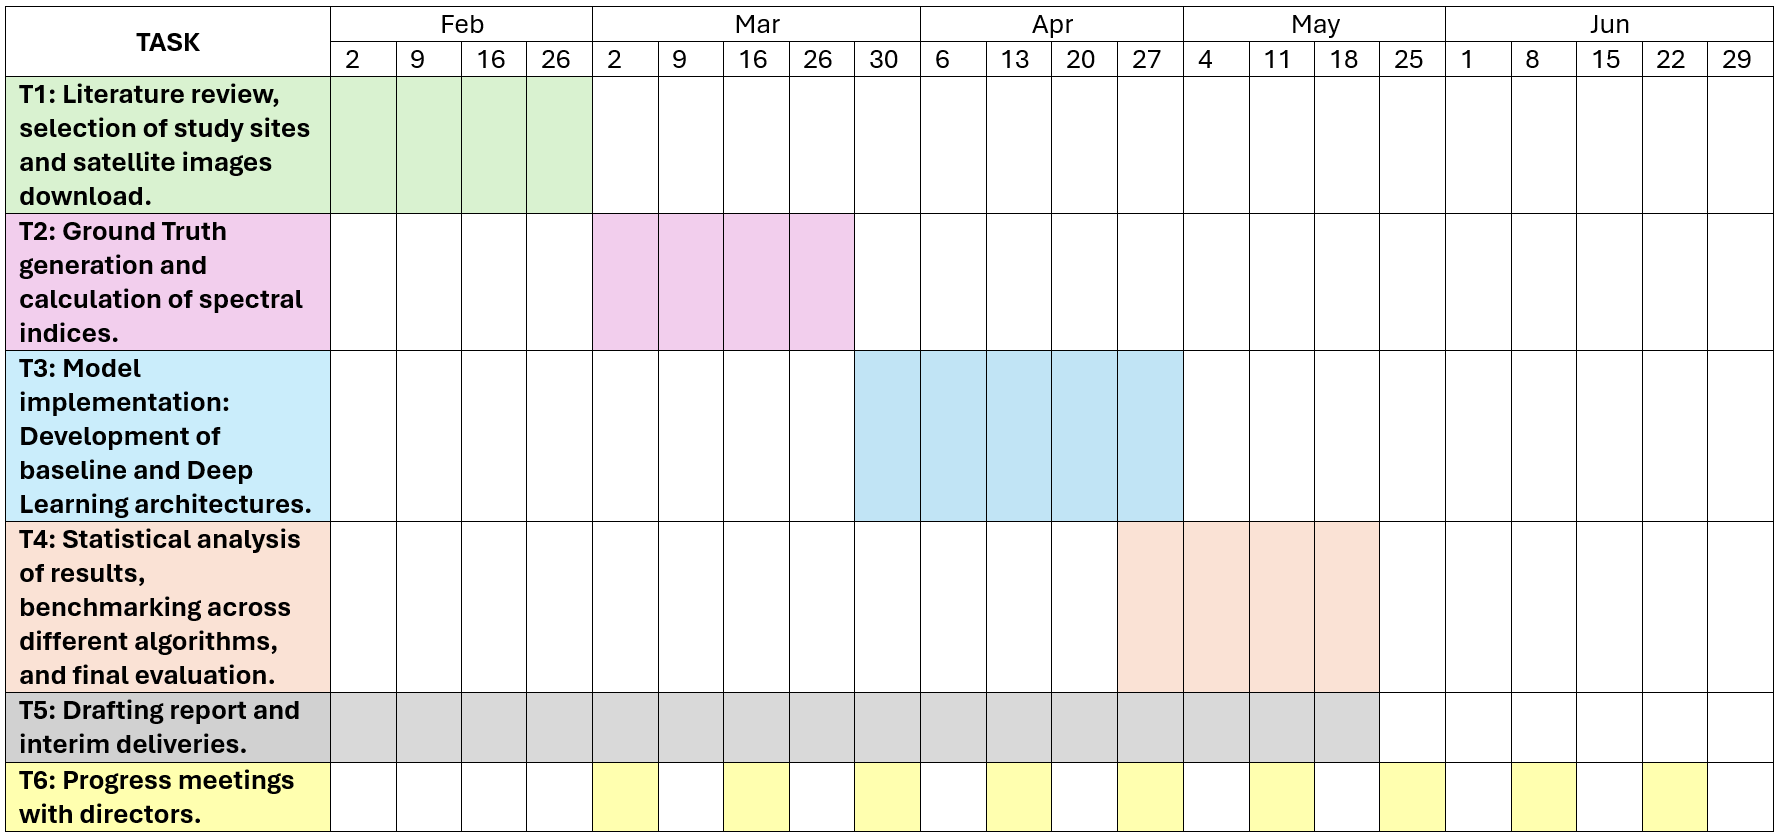
\includegraphics[width=15truecm]{tfm_gantt.png}
    \caption{Gantt chart of the project timeline.}
    \label{fig:gantt}
\end{figure}

\bibliographystyle{apalike}
\bibliography{references}

\end{document}
